\documentclass[11pt]{article}
\usepackage[margin=1in]{geometry}
\usepackage{graphicx,booktabs,amsmath,amssymb,url,microtype,xcolor,caption}
\usepackage[hidelinks]{hyperref}
\usepackage{times}
\captionsetup{font=small,labelfont=bf}
\newcommand{\code}[1]{\texttt{#1}}
\title{\textbf{Exhaustive AI-assisted review of research software finds merged, verified defects in AFNI and SPM,\\ and a thirteen-year-old error in regional homogeneity changes a group result}}
\author{Cynthia Condra\\ \small Unaffiliated \quad \texttt{cindy.krafft@gmail.com}}
\begin{document}
\maketitle

\begin{abstract}
The software behind most published neuroimaging is large, old, mathematically dense, and read far less often than it is run. I asked whether an AI coding agent, directed to read an entire package adversarially and to verify every suspicion by executing code, could find defects that matter, and whether the maintainers would accept the fixes. For AFNI and SPM the answer to both is yes. Reading AFNI's nine numerical subsystems and all eleven of SPM's yielded 36 and 83 confirmed defects respectively, each with file-and-line evidence and a numerical reproduction; the highest-priority ones were sent upstream as ordinary pull requests, each with an issue carrying a runnable reproduction. Within a week the AFNI maintainers had merged two (tie handling in \code{3dReHo}; NIfTI descending slice timing) and the SPM maintainers two (artefact-window baseline offset in \code{@meeg/badsamples}; the sampling rate stamped by \code{spm\_eeg\_downsample}); further fixes are under review and are not reported here until the maintainers have adjudicated them. Only after the code review did I search the literature for exposure, which located five published ReHo studies in the affected regime, whose authors have been contacted, and cleared fifty-two others. To measure what one merged fix means for a published design I re-ran, in AFNI, a pipeline matched step by step to an independent published ReHo analysis of the open UCLA CNP dataset (Cattarinussi et al.\ 2024, DPABI), on 47 participants with schizophrenia and 60 controls, and computed ReHo on identical residuals with the code immediately before and after the fix. Before the fix, \code{3dReHo} decided whether two samples were tied after truncating them to integers, so on percent-signal-change input it returned about a third of the correct value and exactly zero in 9\% of voxels, and the two maps correlated only $r = 0.54$. Because the error scales with each participant's residual amplitude it does not cancel between groups: the before-fix schizophrenia-versus-control map correlated $r = 0.76$ across the brain with the map of where patients' residual amplitude differs from controls', the after-fix map $0.38$; the two builds' $t$-maps correlated 0.57 and changed sign in 30\% of voxels; the global reduction of ReHo in schizophrenia was absent before the fix ($d = 0.01$) and present after it ($d = -0.71$); and under family-wise cluster correction the before-fix build reported increases in temporal pole, hippocampus and cerebellum, exactly where patients' residual amplitude is higher, that the fixed build does not. Both builds and the independent analysis agree on an occipital decrease. The reviews, harnesses, patches, pipeline and results are public.
\end{abstract}

\section{Introduction}
Almost every quantitative result in neuroimaging passes through a few open-source packages that small teams have maintained for decades. The code is excellent and heavily used, and both facts work against complete review: a routine correct for the inputs its author had in mind can be wrong for inputs that became common later, and a test suite cannot cover a regime nobody thought to test. When such a defect surfaces it is treated as a singular event, as with cluster inference \cite{eklund2016} or the platform-dependent chemical-shift scripts in organic chemistry \cite{neupane2019}, rather than as one instance of a class that could be searched for.

Large language models that can read and execute code make the search practical. This paper reports what happened when I pointed one at two of the most used neuroimaging packages, AFNI \cite{cox1996} and SPM, with a simple brief: read everything, assume nothing, and report only what you can reproduce. Two features of the design are deliberate. The review came first and the literature second, so that findings were not filtered by what I expected to matter. And nothing was reported to a maintainer without a numerical reproduction and, where possible, a patch, so that the unit of output is a pull request rather than a list of suspicions. Section~\ref{sec:results} reports what was sent and what the maintainers merged. Section~\ref{sec:reho} then takes one merged fix and asks the question that matters to readers of the affected literature: how much did the results change?

\section{Methods}
\subsection{Exhaustive adversarial review}
An AI coding agent (Claude, Anthropic) worked in a sandboxed environment with the package source checked out, a compiler, and the ability to run code. For each package the source was divided into subsystems and each subsystem was read in full with an adversarial brief: for every routine, what inputs are legal but unanticipated, what happens at boundaries and at zero, where do numeric types change, where is a convention assumed rather than checked. AFNI (\code{afni/afni} master at \code{0488c9e}, 27 August 2026) was divided into nine subsystems where a correctness bug most directly changes a published number: the statistical distribution library, group statistics in C, cluster-extent inference, the single-subject GLM, registration and NIfTI I/O, resting-state and connectivity tools, the R-based group programs, dataset arithmetic, and the Python pipeline with DTI/PCA tools. SPM (\code{spm/spm} development version at \code{530ec52}, 23 August 2026) was divided into eleven: statistical distributions, random field theory and results, the GLM core, spatial preprocessing, file I/O, the C/MEX sources, DCM and Bayesian inversion, numeric and mesh utilities, M/EEG processing, the spatial toolboxes, and the active-inference code. A human directed the agent at the level of package, subsystem and which candidates to pursue; the agent wrote the reviews, harnesses and patches. Every candidate was recorded with file and line evidence.

\subsection{Verification by execution}
No candidate was reported without one of three kinds of execution: compiling the routine under test against an independent or high-precision reference; porting it faithfully, idiosyncrasies included, and testing the port against ground truth on synthetic data; or running the shipped program and observing the defect. In AFNI this meant standalone C harnesses compiled from the actual translation units, comparison against SciPy reference distributions, fuzz tests against sorted references and Monte-Carlo simulation. In SPM it meant Python transcriptions checked against NumPy and SciPy or closed forms, a Monte-Carlo simulation of smooth $\chi^2$ random fields, and, for the fix to \code{spm\_ECdensity}, executing the real MATLAB code in GNU Octave before and after the patch with a new unit test (12 of 23 assertions fail before, 0 after). Candidates that did not survive were recorded as such.

\subsection{Upstream filing}
Findings that survived were ranked by severity times how often the code path runs, and the top of each list was filed in the form each project uses: GitHub issues with runnable reproductions and pull requests carrying the patch and the harness. The maintainers' review is the adjudication.

\subsection{Literature exposure, assessed afterwards}
Exposure was assessed only after the review, and only for the findings at the top of each list, by reading methods sections for the specific trigger of each defect. For the \code{3dReHo} finding this meant a full-text search of Europe PMC for \code{3dReHo} and for ReHo used with AFNI (398 unique records, 310 full texts retrieved) plus every work citing the tool's description \cite{taylor2013}, giving 57 papers that computed ReHo with AFNI, each adjudicated on one question: in what units was the file passed to \code{3dReHo}? For SPM the same after-the-fact reading anchored each Tier-1 finding to the methods papers that document the affected machinery. A separate six-journal full-text survey (44{,}198 articles, 2021--2026; 20{,}501 readable) served as a denominator for how often each package is used, not as the selector of what to read.

\subsection{Reanalysis of the ReHo defect on open data}
\paragraph{Design.} The question is what one merged fix does to a published design, so the pipeline was matched, step by step and before any result was seen, to an independent published ReHo analysis of the same dataset: Cattarinussi et al.\ \cite{cattarinussi2024}, who analysed the UCLA Consortium for Neuropsychiatric Phenomics resting-state data (OpenNeuro ds000030 \cite{poldrack2016}; 3\,T, TR 2\,s, 152 volumes) with DPABI \cite{yan2016} and SPM12 and reported family-wise corrected ReHo differences between schizophrenia and controls. Their published choices, the AFNI analogue used here, and the two deliberate departures are recorded in a plan committed to the repository before the batch ran (\code{analogue\_cattarinussi2024/PLAN.md}); the scoring against their result was fixed in the same plan.

\paragraph{Participants.} All 50 SCHZ participants with a resting run, and every CONTROL participant with a resting run and no lifetime Axis-I diagnosis in the dataset's SCID table (64, of 130), which reconstructs their control group's inclusion rule. One control lacks a T1-weighted image on the OpenNeuro bucket; three of the rest were dropped in the same way as in their pipeline for head motion exceeding 3\,mm or $3^\circ$, as were three SCHZ participants, leaving 60 CONTROL and 47 SCHZ (Table~\ref{tab:demo}). Every exclusion is identical for both builds.

\paragraph{Pipeline.} \code{afni\_proc.py} (AFNI 26.2.06): removal of 10 initial volumes, slice-timing correction, alignment of EPI to the anatomical with AFNI's options for difficult data (\code{lpc+ZZ} cost, \code{-giant\_move}, local EPI unifizing; the default alignment fails on a third of this dataset, see below), affine normalisation to the MNI152 2009 template at 3\,mm, volume registration, tissue segmentation, and the default \code{scale} block to percent signal change; no despiking, no smoothing of the time series, no censoring. Nuisance regression by \code{3dTproject}: the 24-parameter Friston motion model, mean eroded white-matter and CSF series, linear detrending and a 0.01--0.08\,Hz band-pass, matching their Friston-24 plus WM/CSF regression without global-signal regression or scrubbing. \code{3dReHo -nneigh 27} from each build on the identical residuals and mask; each map z-normalised across the participant's brain mask and then smoothed with a 4\,mm Gaussian, as they did, smoothing after rather than before ReHo. The two departures from their pipeline are kept deliberately: percent-signal-change units, because that is the regime in which the defect operates and the one every \code{afni\_proc.py} user is in (the fixed build is unaffected by units), and affine rather than DARTEL normalisation, for compute time. Per-participant quality control recorded the Dice coefficient between the aligned EPI and anatomical masks; with the default alignment options 17 of the first 43 participants processed fell below 0.8 (as low as 0.39, with brain masks half the normal size and displaced), which is why the alignment options above were adopted and the batch restarted before any group result existed. With them no participant fell below 0.8.

\begin{table}[t]
\centering\small
\caption{The 107 participants. Motion is the mean Euclidean norm of the frame-to-frame motion derivative (mm) over all volumes (no censoring). Group comparisons: Student $t$ (df 105) or Fisher's exact test.}
\label{tab:demo}
\begin{tabular}{@{}lccc@{}}
\toprule
 & CONTROL ($n = 60$) & SCHZ ($n = 47$) & $p$ \\
\midrule
Age, years (range) & $30.5 \pm 8.8$ (21--50) & $36.5 \pm 8.8$ (22--49) & 0.001 \\
Sex, F / M & 28 / 32 & 12 / 35 & 0.028 \\
Motion & $0.103 \pm 0.049$ & $0.179 \pm 0.112$ & $<0.001$ \\
Residual SD handed to \code{3dReHo} & $0.329 \pm 0.042$ & $0.357 \pm 0.067$ & 0.008 \\
Voxels the before-fix build returns as zero & 9.6\% & 7.7\% & 0.12 \\
\bottomrule
\end{tabular}
\end{table}

\paragraph{The two builds.} The fix landed in two commits on consecutive days: the tie-detection change itself (\code{94ee52b}, pull request 944) and a guard returning $W = 0$ when the tie correction exactly cancels the denominator (\code{74a90ac}). To isolate the tie-detection change I compare the source immediately before it (\code{4c2bd54}) with the guard applied against master at \code{d202535} (AFNI 26.2.06, bit-identical to the distributed build on test data), so the only difference is whether ties are detected on truncated integers or on floating-point values. A faithful Python port reproduces both builds voxel for voxel to four decimals on synthetic volumes. Releases before 26.2.04 (August 2026) did not close a tie run reaching the end of the sorted series, so in those releases a voxel whose entire series lies inside one integer bin is returned uncorrected, hence correct, rather than as zero; that released build was run as a third arm, and the truncation defect itself is common to every release.

\paragraph{Analysis.} Per participant: the ratio and relative error of before-fix to after-fix ReHo over all in-mask voxels, the fraction of voxels the before-fix build returns as exactly zero, and the voxelwise correlation of the two maps. Group level, on the smoothed z-ReHo maps: \code{3dttest++} two-sample SCHZ versus CONTROL in voxels present in at least 90\% of participants (57{,}207 voxels), no covariates, as in the target analysis; cluster-level inference with \code{3dttest++ -Clustsim} (sign-flip randomisation, 10{,}000 iterations, first-nearest-neighbour, bi-sided) at family-wise $\alpha = 0.05$ for cluster-forming $p = 0.001$, their threshold, and $p = 0.01$, followed by \code{3dClusterize}; clusters labelled with the Neuromorphometrics atlas SPM uses, so that labels are comparable to theirs. The pre-specified score against the target analysis: for each of the nine regions they report (decreases in left superior occipital, right inferior occipital and right postcentral gyri; increases in right anterior orbital and left posterior orbital gyri, bilateral temporal pole, right hippocampus and left cerebellum), whether each build has a corrected cluster of the reported sign inside that region. Two follow-ups were run after the pre-specified result and are labelled as such: the same test with mean motion, and then with whole-brain residual SD, as covariates; and a voxelwise map of where patients' residual amplitude differs from controls' (each participant's residual-SD map z-normalised and smoothed like the ReHo maps, then the same two-sample test), compared with each build's group map.

\section{Results: what was found and what was merged}
\label{sec:results}
Table~\ref{tab:merged} lists the correctness fixes the maintainers have accepted. Further pull requests and issues are open on both projects; they are deliberately not described here, so that the maintainers can adjudicate them before anything is claimed. Behind them stand 36 confirmed findings in AFNI (9 judged capable of changing published numbers, 15 narrower, 12 likely) and 83 in SPM (5 high, 15 medium, 63 low priority), each with file-and-line evidence and a harness in the repository, alongside the code paths that were verified correct, which are recorded with equal care: in SPM the standard fMRI GLM was traced end to end (\code{spm\_spm}, the ReML machinery, the T and F Euler-characteristic densities, both FDR procedures, the NIfTI quaternion core) and held; in AFNI more than forty high-stakes paths held, most verified numerically.

\begin{table}[t]
\centering\small
\caption{Correctness fixes from the AFNI and SPM reviews merged upstream, as of 2 September 2026. Each pull request is paired with an issue carrying a runnable reproduction.}
\label{tab:merged}
\begin{tabular}{@{}llp{8.6cm}l@{}}
\toprule
Package & PR & Change & Merged \\
\midrule
AFNI & 944 & \code{3dReHo}: detect rank ties on the float values, not integer-truncated copies; on percent-signal or standardised input almost every sample had been declared tied and Kendall's $W$ collapsed (Section~\ref{sec:reho}) & 28 Aug 2026 \\
AFNI & 947 & NIfTI reader: loop bound for sequential-descending slice timing compared against the wrong end, so every slice offset was zero and \code{3dTshift} silently did nothing, including on files AFNI itself writes & 28 Aug 2026 \\
SPM & 163 & \code{@meeg/badsamples}: peristimulus baseline added a second time when mapping artefact events to samples, shifting every bad-sample window on epoched data by the baseline length & 2 Sep 2026 \\
SPM & 165 & \code{spm\_eeg\_downsample}: stamp the achieved, not the requested, sampling rate (1000$\to$180\,Hz actually yields 166.7\,Hz) & 2 Sep 2026 \\
\bottomrule
\end{tabular}
\end{table}

Two things about the merged set are worth stating. None was a suspicion: each pull request carried a reproduction the maintainer could run, and in each case the maintainer's comment acknowledged the mechanism (for PR 944, that a mapping from values to ranks ``had not been added''; for PR 947, that descending sequences ``see minimal real-world usage'' despite affecting AFNI's own output). And none would have been found by starting from the literature: no methods section says ``we passed percent-signal data to a routine that truncates to integers.'' The review found the defect; the literature search, done afterwards, found who was exposed.

\subsection{Exposure, found after the fact}
For the \code{3dReHo} defect, 57 papers were adjudicated. Five are potentially affected: two normalised each voxel's series to unit variance, the worst case, and three ran \code{afni\_proc.py} with its default scaling. I do not identify them here. Whether a defect in the software changes a study's conclusions is a question only a rerun by its authors can answer, and the corresponding authors of the five studies have been contacted with the finding, the fix and the reanalysis below. Fifty-two are not, most of them cleared at once by the scaling conventions of the large wrapper pipelines (XCP-D keeps native units; HALFpipe, PhiPipe and CCS grand-mean scale to 10{,}000; C-PAC and DPABI do not call \code{3dReHo}). One paper that L2-normalised its input was first classified as exposed and moved out when the faithful port showed that regime to be exactly correct; that reversal is recorded because it is what verification is for. Eleven papers could not be read. For the SPM findings the exposure is anchored to methods papers rather than to individual studies: the artefact-window defect sits in the machinery documented by the SPM8 M/EEG reference paper, and the free-energy defect in DCM for evoked responses as introduced in its methods papers; a per-paper join for SPM, in the style of the ReHo pass, is future work.


\section{Results: one merged fix, measured end to end}
\label{sec:reho}
\subsection{The defect}
Regional homogeneity \cite{zang2004} is Kendall's coefficient of concordance $W$ over the ranked time series of a voxel and its neighbours, with a correction $\sum_i (t_i^3 - t_i)$ over tie runs of length $t_i$ subtracted from the denominator. In AFNI's implementation \cite{taylor2013} (\code{src/ptaylor/rsfc.c}, lines 63--118) ranks came from a true floating-point sort, but tie \emph{detection} compared values stored into an integer array, so any two samples sharing an integer part were declared tied. For raw scanner units this almost never happens. For percent-signal-change residuals or z-scored series, nearly every sample lies in $(-1, 1)$ and truncates to zero: almost the whole series becomes one tie run, the correction approaches the denominator, and $W$ collapses toward zero, reaching exactly zero in voxels whose whole series lies in one integer bin. Figure~\ref{fig:mech} shows the behaviour of the faithful port against input scale with the 107 participants overlaid. The error is not a constant factor: it depends on the amplitude of each voxel's own series, so the before-fix statistic is partly a measure of BOLD variance; and the affected regime is exactly where \code{afni\_proc.py}'s default \code{scale} block and every ``normalized to unit variance'' step put the data.

\begin{figure}[t]
\centering
\includegraphics[width=\textwidth]{figures/mechanism.pdf}
\caption{\textbf{The defect as a function of input scale.} \textbf{A}, Ratio of before-fix to after-fix ReHo against the SD of the time series handed to \code{3dReHo}, from a faithful port of the routine on Gaussian input (blue: white; green: band-passed 0.01--0.1\,Hz at TR 2\,s), 27-voxel neighbourhoods, 148 time points, 60 simulations per point. Orange: the whole-brain mean ratio for each of the 107 ds000030 participants at the SD of their own residuals. \textbf{B}, The same as relative error. Shaded band: percent-signal-change and z-scored data. Raw scanner units (SD $\gtrsim 5$) are unaffected.}
\label{fig:mech}
\end{figure}

\subsection{Per participant}
Across the 107 participants the residual SD handed to \code{3dReHo} averaged 0.34 (range 0.26--0.66). The before-fix build returned on average 0.35 of the after-fix whole-brain mean ReHo (0.080 versus 0.231; range 0.19--0.66), a relative error over all voxels of 64\% (range 35--79\%); it returned exactly zero in a mean 9\% of in-mask voxels (range 0--35\%) and about 0.41 of the correct value elsewhere. The error tracks residual amplitude across participants ($r = -0.91$). The before- and after-fix maps correlated $r = 0.54$ across voxels (range 0.25--0.85), the correlation rising with residual SD ($r = 0.67$; Fig.~\ref{fig:re}B). The released build returned 0.81 of the correct value and maps correlating $r = 0.91$, because on unsmoothed residuals many voxels' series lie inside one integer bin and are returned uncorrected. The defect reorders voxels rather than rescaling them, to a degree that varies with each participant's signal amplitude.

\subsection{Between groups}
With no censoring, the patients' residual amplitude is \emph{higher} than the controls' (Table~\ref{tab:demo}; they move more), so the bias is group-dependent and now favours the patients. Table~\ref{tab:group} and Figure~\ref{fig:re}C give the contrasts. The $t$-maps from the two builds correlated 0.57, disagreed in sign in 30\% of voxels, and their $p<0.001$ sets shared 38 of 576 voxels. The whole-brain mean reduction of ReHo in schizophrenia, the simplest statistic such papers report and the one the meta-analytic literature supports, is absent under the before-fix build ($t(105) = 0.04$, $p = 0.97$, $d = 0.01$) and present under the after-fix build ($t = -3.64$, $p < 0.001$, $d = -0.71$) and the released build ($t = -4.97$, $d = -0.96$), on identical residuals.

\begin{table}[t]
\centering\small
\caption{SCHZ versus CONTROL (47 vs 60, \code{3dttest++} on smoothed z-ReHo, 57{,}207-voxel mask), same participants and residuals, the only difference being which \code{3dReHo} produced the input maps. Cluster inference: \code{3dttest++ -Clustsim}, 10{,}000 sign-flip randomisations, NN1, bi-sided, $\alpha = 0.05$; labels from the Neuromorphometrics atlas at the peak; $+$ SCHZ $>$ CONTROL, $-$ SCHZ $<$ CONTROL.}
\label{tab:group}
\setlength{\tabcolsep}{4pt}\begin{tabular}{@{}p{4.6cm}p{5.7cm}p{4.6cm}@{}}
\toprule
 & Before fix (\code{4c2bd54}) & After fix (26.2.06) \\
\midrule
Voxels $|t|>3.39$ ($p<.001$) & 384 (170 $-$, 214 $+$) & 230 (126 $-$, 104 $+$) \\
Corrected clusters, $p<.001$ & 5: L calcarine ($-$, 75), L calcarine/occipital pole ($-$, 42), R temporal pole ($+$, 40), R superior frontal ($+$, 37), L cerebellum ($+$, 33) & 2: L cuneus/occipital pole ($-$, 33), L calcarine ($-$, 33) \\
Corrected clusters, $p<.01$ & 6: L calcarine ($-$, 518), R cerebellum ($+$, 156), R postcentral ($-$, 155), L cerebellum ($+$, 150), L superior frontal ($+$, 146), R hippocampus ($+$, 136) & 1: L cuneus/calcarine ($-$, 313) \\
\midrule
Spatial correlation of $t$-maps & \multicolumn{2}{c}{0.57} \\
Voxels where $t$ changes sign & \multicolumn{2}{c}{30\%} \\
Overlap of $p<.001$ sets (before $\cap$ after / $\cup$) & \multicolumn{2}{c}{38 / 576} \\
Overlap of corrected clusters, $p<.001$ / $p<.01$ & \multicolumn{2}{c}{42 / 251 \quad 160 / 1{,}414} \\
Global mean ReHo, SCHZ $-$ CONTROL & $d = 0.01$, $p = 0.97$ & $d = -0.71$, $p < 0.001$ \\
\bottomrule
\end{tabular}
\end{table}

\subsection{Cluster-level inference and the independent analysis}
Table~\ref{tab:group} lists the family-wise corrected clusters. Both builds find reduced ReHo in schizophrenia in calcarine cortex and the occipital pole; the before-fix build additionally finds increases in right temporal pole, right superior frontal gyrus and left cerebellum at $p < 0.001$, and in right hippocampus and both cerebellar hemispheres at $p < 0.01$, none of which the fixed build finds at either threshold. Corrected clusters share 42 of 251 voxels at $p < 0.001$, the calcarine cluster.

Against the nine regions of the independent DPABI analysis, the pre-specified score is in Table~\ref{tab:score}. Both builds reproduce the occipital decrease (our peaks fall in calcarine cortex and cuneus rather than in the superior and inferior occipital gyri as labelled, so the strict score does not credit it). Only the before-fix build reproduces the increases: right temporal pole and left cerebellum at $p < 0.001$, plus right hippocampus and right postcentral at $p < 0.01$. The fixed build reproduces no increase. On this score the defective build agrees with the independent analysis better than the fixed one.

\begin{table}[t]
\centering\small
\caption{Pre-specified score against the nine regions Cattarinussi et al.\ \cite{cattarinussi2024} report for SCHZ versus HC (decreases: L superior occipital, R inferior occipital, R postcentral; increases: R anterior orbital, L posterior orbital, bilateral temporal pole, R hippocampus, L cerebellum).}
\label{tab:score}
\begin{tabular}{@{}lccc@{}}
\toprule
Build & mean $t$ of the reported sign & corrected cluster of the reported sign, $p<.001$ & $p<.01$ \\
\midrule
Before fix & 9 / 9 & 2 / 9 & 4 / 9 \\
After fix & 8 / 9 & 0 / 9 & 0 / 9 \\
Released (pre-26.2.04) & 7 / 9 & 0 / 9 & 0 / 9 \\
\bottomrule
\end{tabular}
\end{table}

\subsection{Why the defective build agrees: amplitude, not synchrony}
Two labelled follow-ups changed nothing: with mean motion as a covariate, and with whole-brain residual SD as a covariate, every before-fix cluster survived with the same peak and size (as expected for the second, since the maps are z-normalised per participant and the effect is regional). The third follow-up locates the effect (Fig.~\ref{fig:amp}). The map of where patients' residual amplitude differs from controls' correlates $r = 0.76$ across the 57{,}207-voxel mask with the before-fix group map and $r = 0.38$ with the after-fix map; the difference between the two builds' maps correlates $r = 0.45$ with it. Inside the before-fix SCHZ $>$ CONTROL clusters at $p < 0.001$ (temporal pole, superior frontal, cerebellum) the amplitude map averages $t = +2.5$, against $-0.2$ over the rest of the mask; inside the SCHZ $<$ CONTROL clusters of either build (calcarine) it averages $-3.4$ and $-3.2$. The before-fix group map is largely a map of where the patients' residual amplitude differs, and the clusters that matched the independent analysis sit precisely where their amplitude is higher: the low-signal regions of temporal pole, orbitofrontal cortex, hippocampus and cerebellum, in a patient group that moves more, in a design that neither censors nor covaries motion. This is the defect's mechanism operating at the group level: the truncated-tie statistic turns a regional amplitude difference into an apparent synchrony increase. The fixed build, on identical residuals, does not produce it.

\begin{figure}[t]
\centering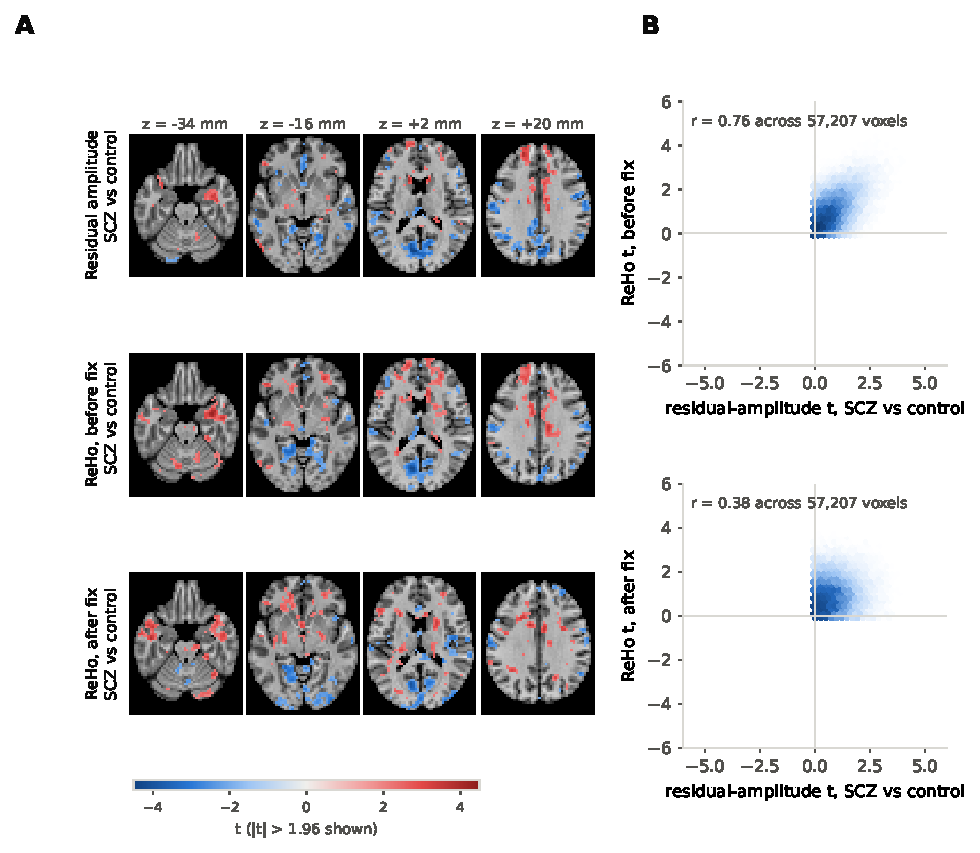
\includegraphics[width=\textwidth]{figures/amplitude.pdf}
\caption{\textbf{The defect's amplitude dependence at the group level.} \textbf{A}, SCHZ-versus-CONTROL $t$-maps ($|t| > 1.96$ shown, four axial slices, 90\%-coverage mask) for residual amplitude (each participant's residual-SD map, z-normalised and smoothed like the ReHo maps), for before-fix z-ReHo, and for after-fix z-ReHo. \textbf{B}, Voxelwise density of the before-fix (top) and after-fix (bottom) ReHo $t$ against the residual-amplitude $t$, with the correlation across the mask.}
\label{fig:amp}
\end{figure}

\begin{figure}[p]
\centering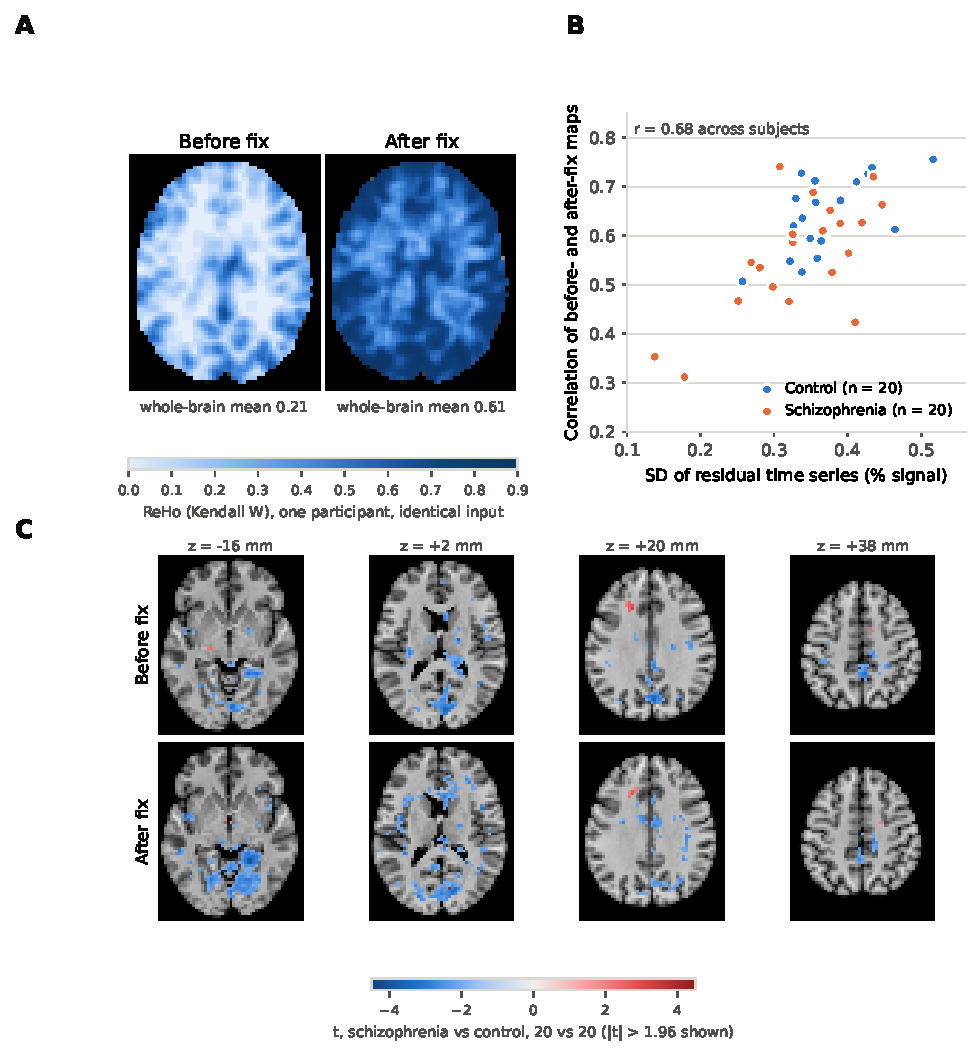
\includegraphics[width=0.92\textwidth]{figures/reanalysis.pdf}
\caption{\textbf{One defect, before and after, on identical data.} \textbf{A}, ReHo for one control participant computed from the same residual time series by the before-fix \code{3dReHo} (left) and the after-fix build (right), same slice and colour scale. The before-fix values are about a third of the correct ones, exactly zero in 7.4\% of this participant's mask (the palest regions), and differently arranged. \textbf{B}, For each of 107 participants, the voxelwise correlation between before- and after-fix maps against the SD of that participant's residuals. \textbf{C}, SCHZ-versus-CONTROL $t$-maps (47 vs 60) from the before- and after-fix z-ReHo maps, $|t|>1.96$ shown, four axial slices, 90\%-coverage mask.}
\label{fig:re}
\end{figure}

\section{Discussion}
\paragraph{What the case study establishes.} Every ReHo map computed by AFNI on percent-signal-change or standardised input before 27 August 2026 was affected, and not in the benign way of a wrong scale factor. In a typical participant the before-fix map was a third of the correct value with a different spatial arrangement and a tenth of the brain at zero; between groups whose signal amplitude differs, as clinical groups typically do, the before-fix statistic mixes a synchrony difference with an amplitude difference. In a design matched to a published analysis of the same data, that mixing produced family-wise corrected clusters of apparently increased synchrony in schizophrenia exactly where the patients' residual amplitude is higher, clusters the fixed build does not produce, and erased the global reduction of ReHo in schizophrenia that the fixed build and the literature both show. That the defective build agreed \emph{better} with the independent analysis on a region count is the most instructive result here: agreement between two unadjusted analyses is not evidence of correctness when the defect and the confound point the same way, and the amplitude map shows which way they point. I make no claim about the conclusions of the five potentially affected studies, which is why they are not named; none shares its data, and only reruns by their authors, who have been contacted, can settle what changes. Nor about the independent analysis: DPABI's ReHo does not have this defect, and whether its increases in those regions are amplitude-driven cannot be decided from here. The reanalysis is of their design, on open data, with nothing but the fix varied, and it says the reruns are worth doing. Its limits: one dataset, one configuration, affine rather than nonlinear normalisation, and no covariates in a sample whose groups differ in age, sex and motion, so that the clinical contrast is a vehicle for the between-build comparison rather than a finding about schizophrenia. It isolates the tie-detection change given the concurrent divide-by-zero guard; the released code left the lowest-amplitude voxels uncorrected rather than zeroed, which on unsmoothed residuals makes its error much smaller (0.81 of the correct value) but leaves the same amplitude dependence, and it too shows the global reduction the \code{4c2bd54} build erases.

\paragraph{Why review-first matters.} Each of the four merged defects was invisible from the literature side. A methods section does not say which loop bound the NIfTI reader compared against, whether the artefact detector and the artefact reader agreed about the baseline, or whether a sampling rate was requested or achieved. Starting from the papers, as reproducibility efforts usually do, would have found none of them. Starting from the code found all four, and the literature pass afterwards found who was exposed, including a reversal (the L2-normalised regime) that only the faithful reproduction could have produced.

\paragraph{Why the defects survived.} Each routine was correct for the data its author tested it on; the regime in which it fails was created later, by another program's default, by a rarely used slice order, by an epoching convention, by a non-integer ratio. No unit test exercised the regime (\code{spm\_ECdensity} had none at all) and no user could see a defect whose signature is ``lower ReHo everywhere, more so in noisier participants.'' This is the general shape of the findings: not carelessness but the combinatorics of large, old codebases and evolving conventions, which no team can read exhaustively with the question ``what if the input is small, or tied, or descending'' in mind for every line.

\paragraph{What machine-assisted review changes.} That question is now cheap to ask of every line. Two features of the method are essential and I would caution against dropping either. Verification by execution is what separates a finding from a plausible story; a substantial fraction of the agent's candidates did not survive it. And upstream review is the adjudication: the merged fixes are the deliverable, and the maintainers' reading of a patch, not ours, is what makes it trustworthy. Given both, the economics change: an exhaustive adversarial read of AFNI or SPM, with a numerical check of each suspicion, costs days of compute rather than years of expert time, and its output arrives in the form maintainers already accept.

\paragraph{Recommendations.} Funders and journals should treat audits of the software behind published results as reproducibility infrastructure rather than as one-off events. Maintainers should be resourced to receive and review such reports, because a verified finding has value only once it is a merged fix and a corrected literature. And authors should publish their analysis scripts together with the exact versions of every piece of software they ran. The 57-paper exposure pass here took days of reading and still left eleven papers unresolved, because methods sections say ``ReHo was computed in AFNI'' and not which build, in which units, with which options; a published script and version string answer all three at once. Software will keep having bugs. Whether the literature can be corrected when one is found depends on whether it is possible to tell, quickly and mechanically, who ran the affected code, and today it mostly is not.

\paragraph{Limitations.} ``Confirmed'' means traced end to end and reproduced as stated, not adjudicated by the maintainers; where they disagree, their reading wins. The SPM Tier-1 fixes other than \code{spm\_ECdensity} were verified by transcription and reasoning rather than by executing MATLAB, which is stated in each pull request. Exposure was assessed only for the top findings, and for SPM only at the level of methods papers. The literature pass reaches only openly readable full text, so a paywalled paper that says ``ReHo was computed in AFNI'' is invisible to it. The same repository holds reviews of seven further packages at varying stages of verification and filing; they are not reported here because their fixes have not yet been through maintainer review.

\section*{Data and code availability}
The component reviews, every verification harness, the patches and issue texts, the reanalysis pipeline (\code{analogue\_cattarinussi2024/}: pre-registered plan, \code{run\_subject\_dpabi.sh}, \code{group\_analysis\_dpabi.sh}, \code{score\_targets.py}, the follow-up scripts), subject lists, per-participant tables, group $t$-maps and figures are at \url{https://github.com/cindykrafft/research-software-audit}. Imaging data are OpenNeuro ds000030. The \code{3dReHo} builds are reproducible from \code{afni/afni} at \code{4c2bd54} (plus \code{74a90ac}) and \code{d202535}. Merged pull requests: \url{https://github.com/afni/afni/pull/944}, \url{https://github.com/afni/afni/pull/947}, \url{https://github.com/spm/spm/pull/163}, \url{https://github.com/spm/spm/pull/165}.

\section*{Disclosure of AI use}
The code reviews, harnesses and patches described here were produced by an AI coding agent (Claude, Anthropic) operating under the author's direction; every reported finding was verified by executing code, and every upstream filing was reviewed by the author before submission. The same system assisted in drafting this manuscript and produced its figures from the checked-in results. The author has no financial interest in any software named.

\begin{thebibliography}{99}
\bibitem{eklund2016} Eklund A, Nichols TE, Knutsson H. Cluster failure: why fMRI inferences for spatial extent have inflated false-positive rates. \emph{Proc Natl Acad Sci USA} 113:7900--7905 (2016).
\bibitem{neupane2019} Bhandari Neupane J, Neupane RP, Luo Y, Yoshida WY, Sun R, Williams PG. Characterization of leptazolines A--D, polar oxazolines from the cyanobacterium \emph{Leptolyngbya} sp., reveals a glitch with the ``Willoughby--Hoye'' scripts for calculating NMR chemical shifts. \emph{Org Lett} 21:8449--8453 (2019).
\bibitem{cox1996} Cox RW. AFNI: software for analysis and visualization of functional magnetic resonance neuroimages. \emph{Comput Biomed Res} 29:162--173 (1996).
\bibitem{taylor2013} Taylor PA, Saad ZS. FATCAT: (an efficient) functional and tractographic connectivity analysis toolbox. \emph{Brain Connect} 3:523--535 (2013).
\bibitem{poldrack2016} Poldrack RA, Congdon E, Triplett W, et al. A phenome-wide examination of neural and cognitive function. \emph{Sci Data} 3:160110 (2016). OpenNeuro ds000030.
\bibitem{cattarinussi2024} Cattarinussi G, Di Camillo F, Grimaldi DA, Sambataro F. Diagnostic value of regional homogeneity and fractional amplitude of low-frequency fluctuations in the classification of schizophrenia and bipolar disorders. \emph{Eur Arch Psychiatry Clin Neurosci} (2024). doi:10.1007/s00406-024-01838-4.
\bibitem{yan2016} Yan CG, Wang XD, Zuo XN, Zang YF. DPABI: Data Processing \& Analysis for (Resting-State) Brain Imaging. \emph{Neuroinformatics} 14:339--351 (2016).
\bibitem{zang2004} Zang Y, Jiang T, Lu Y, He Y, Tian L. Regional homogeneity approach to fMRI data analysis. \emph{NeuroImage} 22:394--400 (2004).
\end{thebibliography}
\end{document}
